\section{Expected Utilization with $RTT$ as a random variable}
  In order to see how cross traffic burstiness impacts Rapid throughput, we 
  study the overall link utilization, given by:
  \begin{equation}
    U = \frac{R_{avg} + R}{C}
    \label{util}
  \end{equation}
  Replacing equation \eqref{ravg} for $R_{avg}$ and the equations for $R$ 
  derived in section 2 and 3, the link utilization can be expressed as a 
  function of $T_{on}$, $T_{off}$, $R_{on}$, $C$, $\tau$, $\eta$, and $RTT$. 
  Figure \ref{utilvsrtt} shows a plot of the utilization $U$ as a function of 
  $RTT$ after replacing $T_{on} = 25 ms$, $T_{off} = 100 ms$, 
  $R_{on} = 500 Mbps$, $C = 1Gbps$, $\tau = 7.5 ms$, and $\eta = 7 ms$. The 
  horizontal line around 0.95 is the worst case utilization value obtained 
  using the models derived in \cite{Lovewell2011-Noise-TR}. If we treat 
  $RTT$ as a random variable, we can use the utilization function of Figure 
  \ref{utilvsrtt} to compute the expected value of utilization.
  \begin{figure}[h]
    \centering
    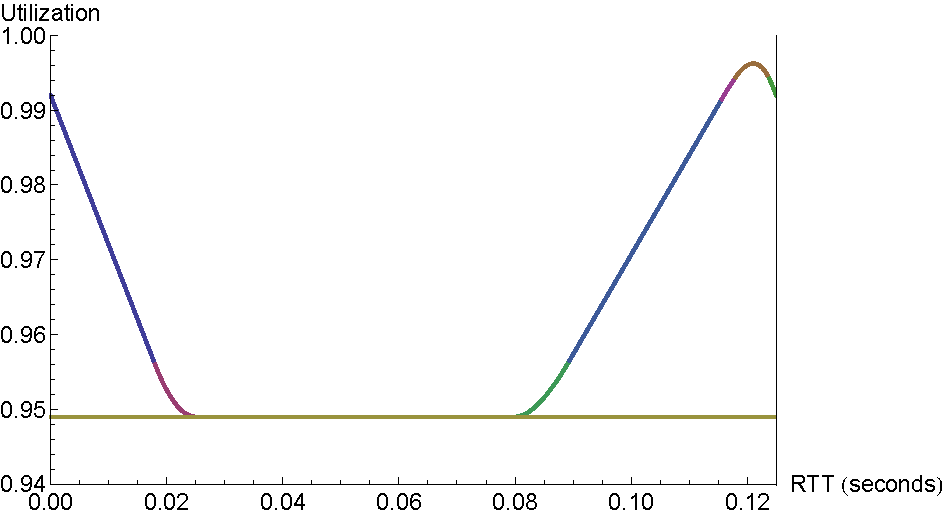
\includegraphics[width=0.9\textwidth]{img/utilvsrtt.pdf}
    \caption{Utilization vs RTT}
    \label{utilvsrtt}
  \end{figure}

  We use the models we have developed to quantitatively study the impact that 
  cross traffic burstiness can have on Rapid and the extend to which it can 
  be alleviated. From \cite{Lovewell2011-Noise-TR} we learned that the 
  inability of Rapid to fully utilize the bottleneck link due to large-scale 
  cross traffic bursts:
  \begin{enumerate}
    \item does not depend individually on $\tau$ or $\eta$, but rather on 
    $\tau - \eta$, the difference between the two smoothing parameters.

    \item is proportional to the relative load of the cross traffic 
    $\frac{R_{avg}}{C}$.

    \item is proportional to the ratio $\frac{T_{off}}{T_{on}}$.
  \end{enumerate}

  For the remainder of this section, we treat $RTT$ as a uniform random 
  variable with probability density function:
  \begin{equation}
    f_{RTT}(RTT) =
    \begin{cases}
        \frac{1}{T_{on} + T_{off}} & \text{if } 0 < RTT < T_{on} + T_{off} \\
        0 & \text{otherwise}
    \end{cases}
    \label{rttpdf}
  \end{equation}

  \subsection{Role of $\tau - \eta$}
    Figure \ref{rtttaueta} plots the expected utilization as a function of 
    $\tau - \eta$. $C$ is set to $1Gbps$ and the different curves correspond 
    to different values of $T_{on}$, $T_{off}$, and $R_{avg}$. The expected 
    utilization is slightly better than the worst case utilization found in 
    \cite{Lovewell2011-Noise-TR}. We find similar results as in 
    \cite{Lovewell2011-Noise-TR}:
    \begin{itemize}
      \item Expected utilization  decreases with increase in $\tau - \eta$.
      \item The loss in expected utilization due to large $\tau - \eta$ is 
      influenced somewhat, but not significantly, by the values of $R_{avg}$, 
      $T_{on}$, and $T_{off}$.
      \item For a given value of $\tau - \eta$, a larger value of $\tau$ seems 
      to alleviate the loss in expected utilization due to cross-traffic 
      burstiness.
    \end{itemize}
    \begin{figure}[h]
      \centering
      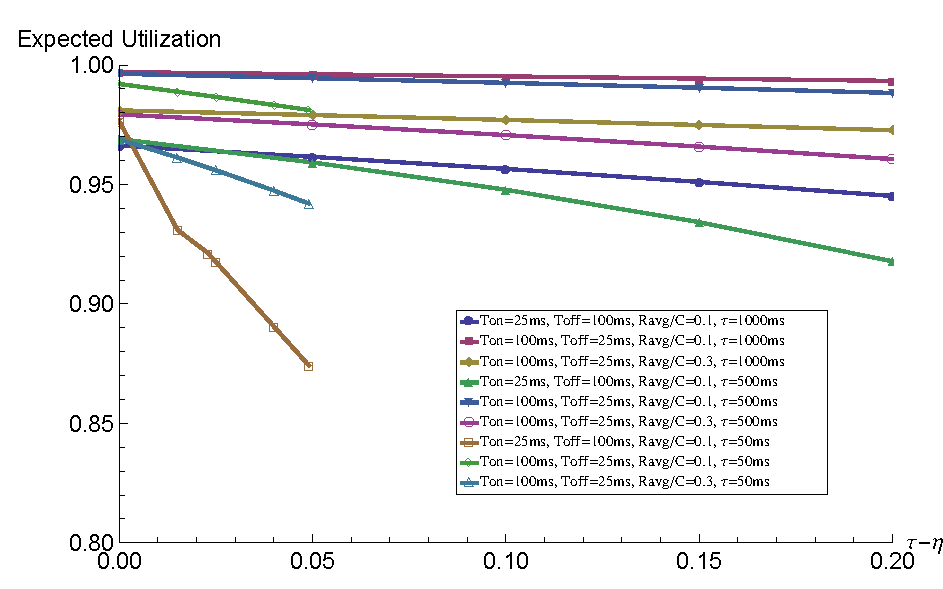
\includegraphics[width=0.9\textwidth]{img/rtttaueta.pdf}
      \caption{Role of $\tau - \eta$}
      \label{rtttaueta}
    \end{figure}

  \subsection{Role of $\frac{R_{avg}}{C}$}
    Figure \ref{rttravgc} plots the expected utilization as a function of 
    $\frac{R_{avg}}{C}$. The different curves correspond to 4 different 
    values of $(T_{on}, T_{off})$ and 2 values of 
    $\tau$ ($\tau - \eta = 1ms$). Again, the expected utilization is slightly 
    better than the worst case utilization and the results are simulart as the 
    ones in \cite{Lovewell2011-Noise-TR}:
    \begin{itemize}
      \item The expected utilization decreases with increase in 
      $\frac{R_{avg}}{C}$. This trend is more pronounced for smaller values of 
      $\frac{T_{on}}{T_{off}}$.
      \item For a given combination of $T_{on}$ and $T_{off}$, Rapid performs 
      better when bursts are "small-scale" ($\tau$, $\eta$ are sufficiently 
      larger thatn $T_{on}$, $T_{off}$). As long as the bursts are 
      small-scale, the value of $\tau$ dpes not influence Rapid performance 
      much. Using large value of $\tau$ and $\eta$ can help ensure the 
      bursts are relatively "small" in scale and Rapid performs well.
    \end{itemize}
    \begin{figure}[h]
      \centering
      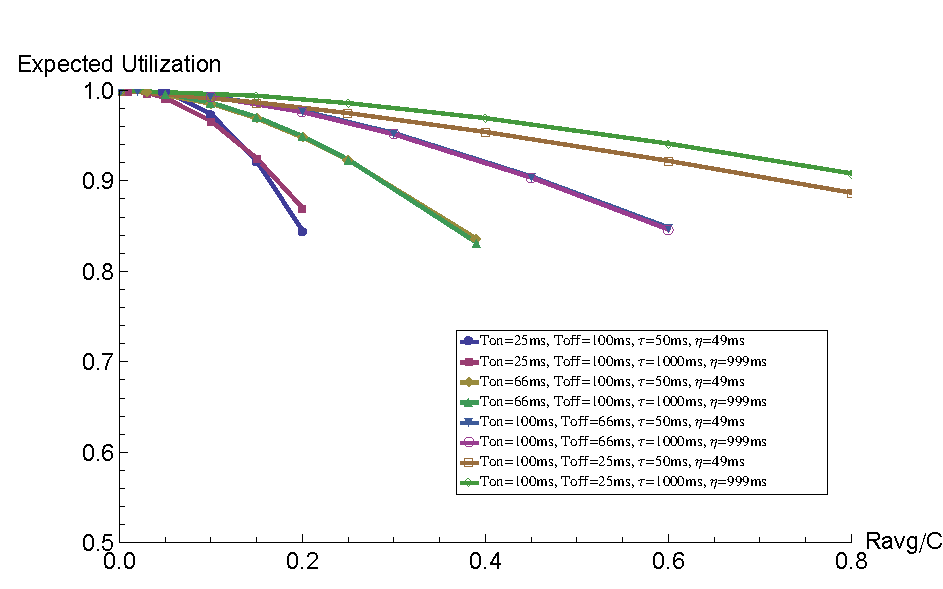
\includegraphics[width=0.9\textwidth]{img/rttravgc.pdf}
      \caption{Role of $\frac{R_{avg}}{C}$}
      \label{rttravgc}
    \end{figure}

  \subsection{Role of $\frac{T_{on}}{T_{off}}$}
    \begin{figure}[h]
      \centering
      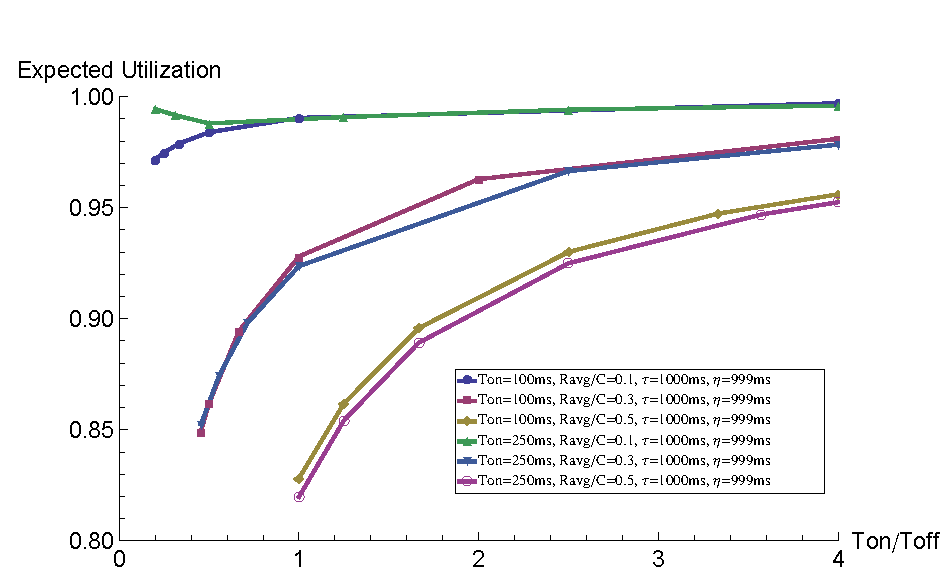
\includegraphics[width=0.9\textwidth]{img/rtttontoff.pdf}
      \caption{Role of $\frac{T_{on}}{T_{off}}$}
      \label{rtttontoff}
    \end{figure}

